\documentclass{beamer}

\usepackage{geometry} % Pour passer au format A4
\usepackage{graphicx} % Required for including pictures
\usepackage{float} %

\usepackage{amsmath,amsfonts,amssymb,amsthm}
\usepackage[T1]{fontenc}
\usepackage[english,francais]{babel}
\usepackage[utf8]{inputenc}
\usepackage{lmodern}
\usepackage{eurosym} % signe Euros
\usepackage{verbatim}
\usepackage{multicol}
\usepackage{textcomp}
\usefonttheme[onlymath]{serif}
\usetheme{m} 

\title{{\rmfamily{\textsc{C}}}osinus d'un angle dans un triangle rectangle}

\begin{document}

\frame{\titlepage}

\section{{\rmfamily{\textsc{I - L}}}a formule}

\begin{frame}
  \frametitle{{\rmfamily{\textsc{I - L}}}a formule}

  \begin{block}{}
    1) Dans un triangle \textbf{rectangle}.
    $$\text{cosinus d'un angle} = \dfrac{\text{longueur de l'adjacent à l'angle}}{\text{longueur de l'hypoténuse}}$$ 
  \end{block}

  \begin{multicols}{2}
    \begin{block}{} 
      2) EFG est un triangle \textbf{rectangle} en E.\\
      $\cos(\overbrace{EFG}) = \dfrac{FE}{FG}$
    \end{block}

    
    \begin{figure}[H]
	    \centering
	    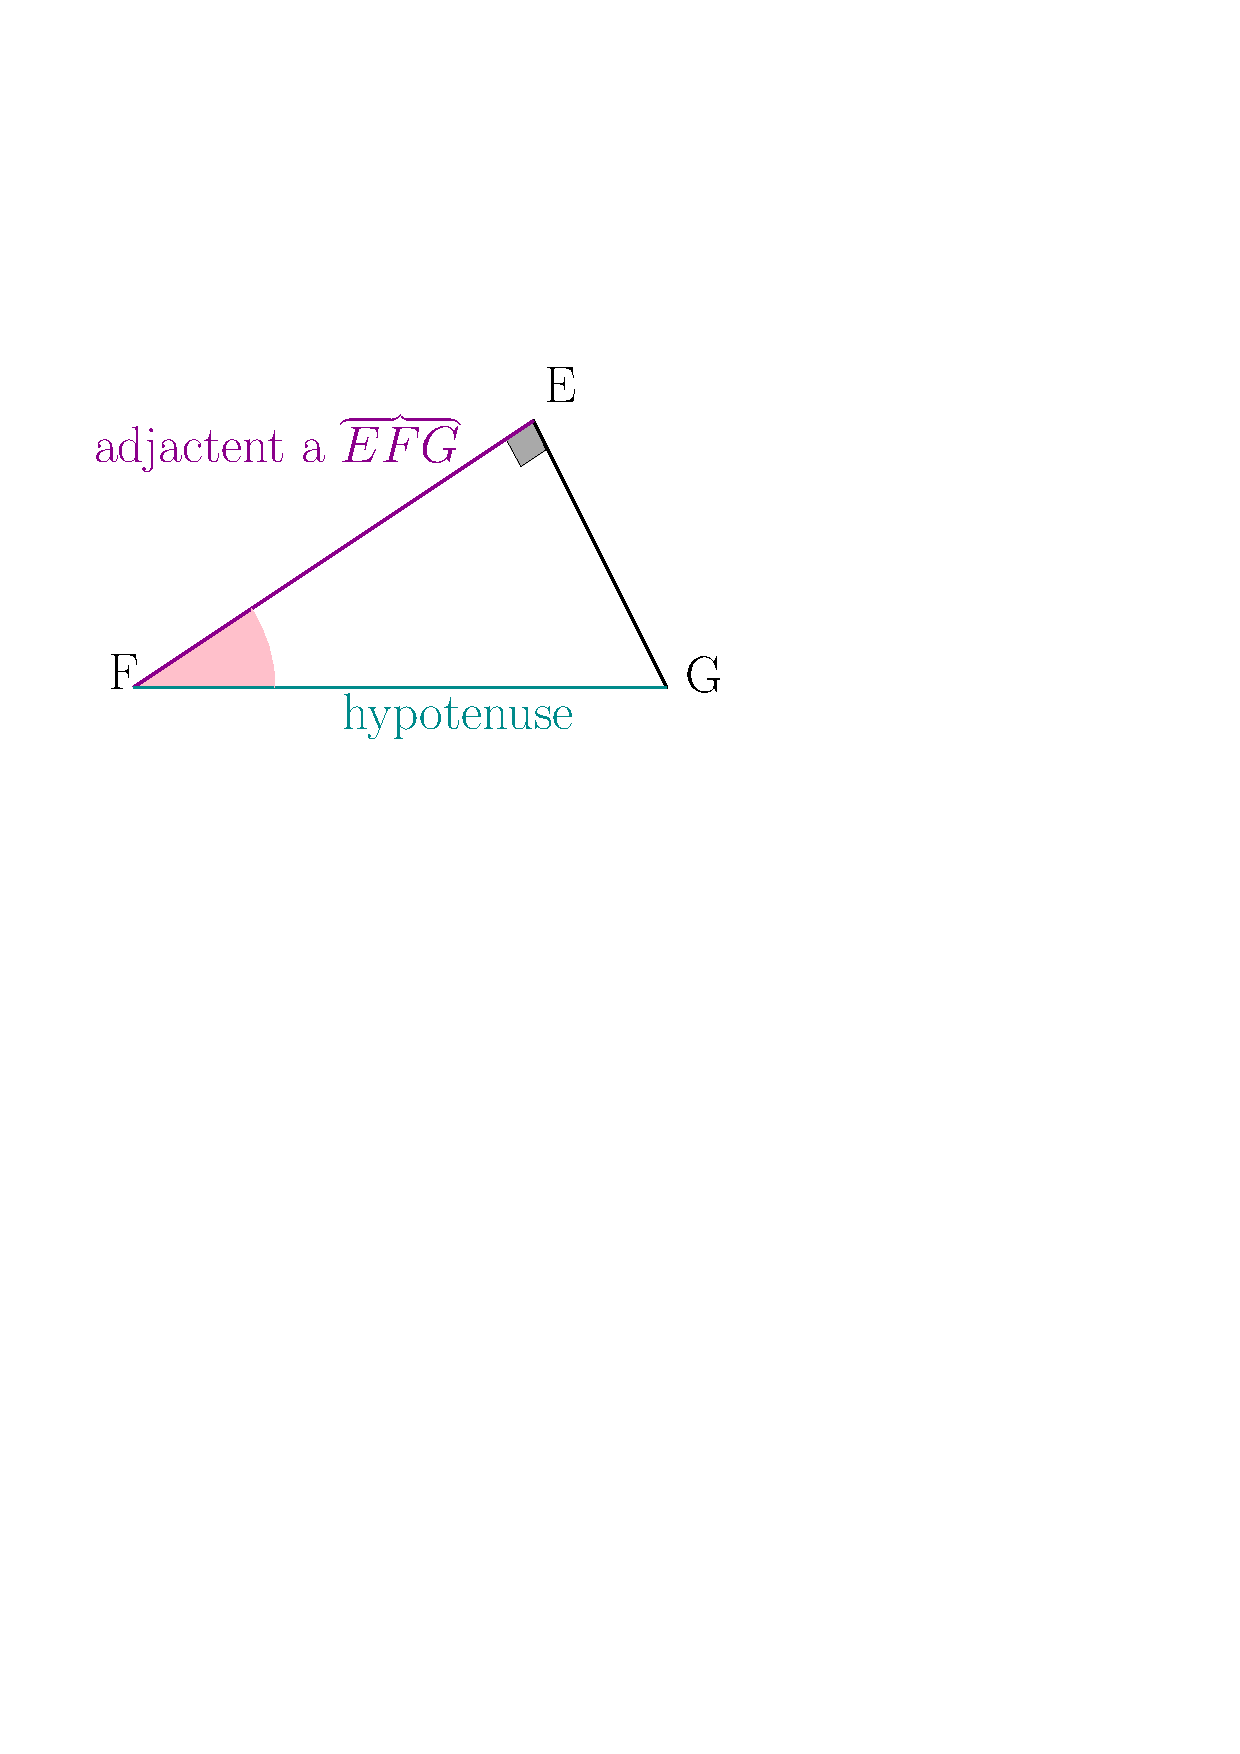
\includegraphics[width=\linewidth]{sources/2/tri-EFG.pdf}
	  \end{figure}
  \end{multicols}
\end{frame}

\begin{frame}
  \frametitle{{\rmfamily{\textsc{I - L}}}a formule}
  
  \begin{block}{Remarques}
    \begin{itemize}
    \item La lettre au centre de l'angle se répète deux fois dans la formule du cosinus.
    \item Le cosinus d'un angle dans un triangle rectangle est toujours compris entre 0 et 1.
    \end{itemize}
  \end{block}
  
\end{frame}


\section{{\rmfamily{\textsc{II - U}}}sages}

\begin{frame}
  \frametitle{{\rmfamily{\textsc{II - U}}}sages}

  A) Trouver une longueur manquante dans un triangle rectangle
  
  \begin{exampleblock}{a. Recherche de l'adjacent}
    
    \begin{multicols}{2}
      \begin{figure}[H]
	      \centering
	      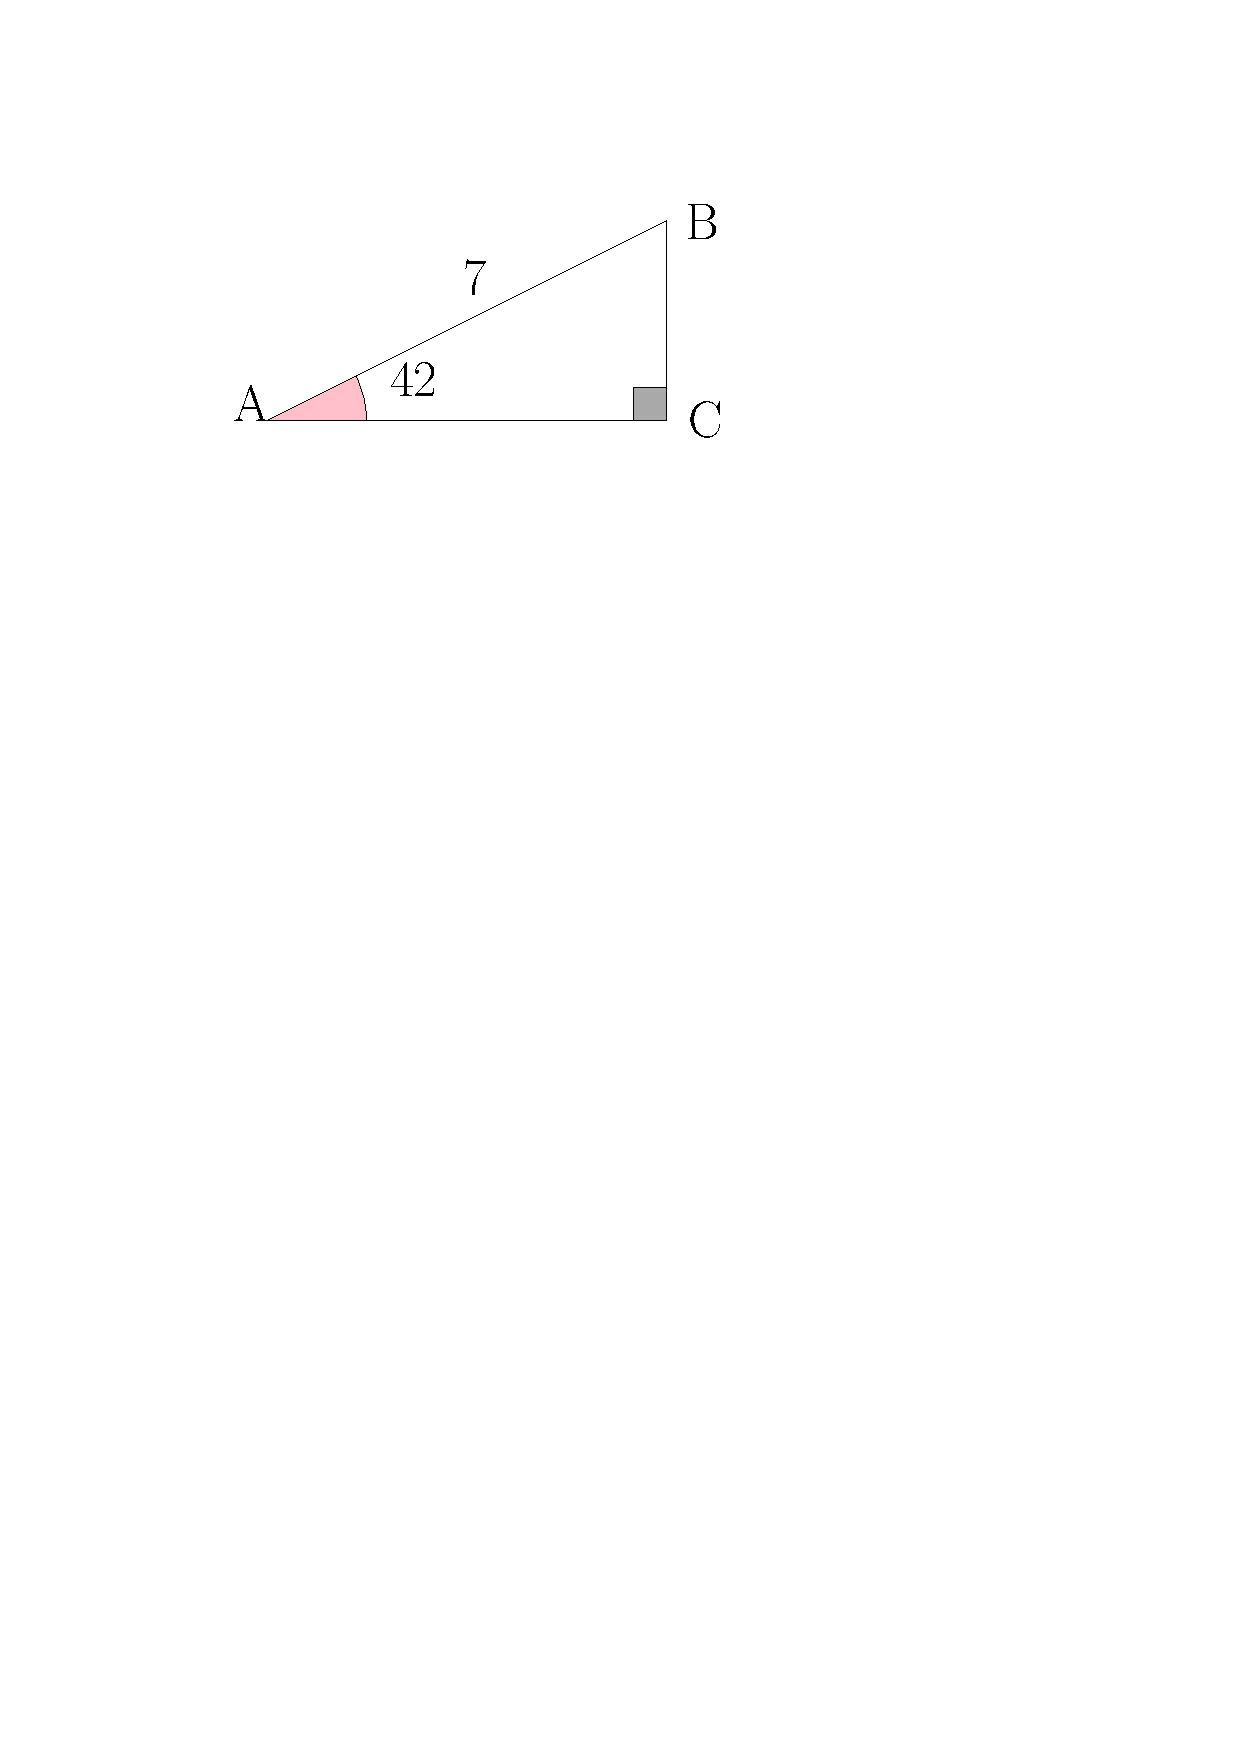
\includegraphics[width=\linewidth]{sources/2/rec-a1.pdf}
	    \end{figure}
      
      \vspace{.5cm}
      
      ABC est un triangle rectangle en C.\\
      
      $\cos(\overbrace{CAB}) = \dfrac{AC}{AB}$\\
      $\cos(42) = \dfrac{AC}{7}$\\
      $AC = 7 \times \cos(42)$\\
      $AC \approx 5.2$
      
    \end{multicols}
  \end{exampleblock}
  
\end{frame}

\begin{frame}
  \frametitle{{\rmfamily{\textsc{II - U}}}sages}
  
  \begin{exampleblock}{b. Recherche de l'hypoténuse}
    
    \begin{multicols}{2}
      
      \begin{figure}[H]
	      \centering
	      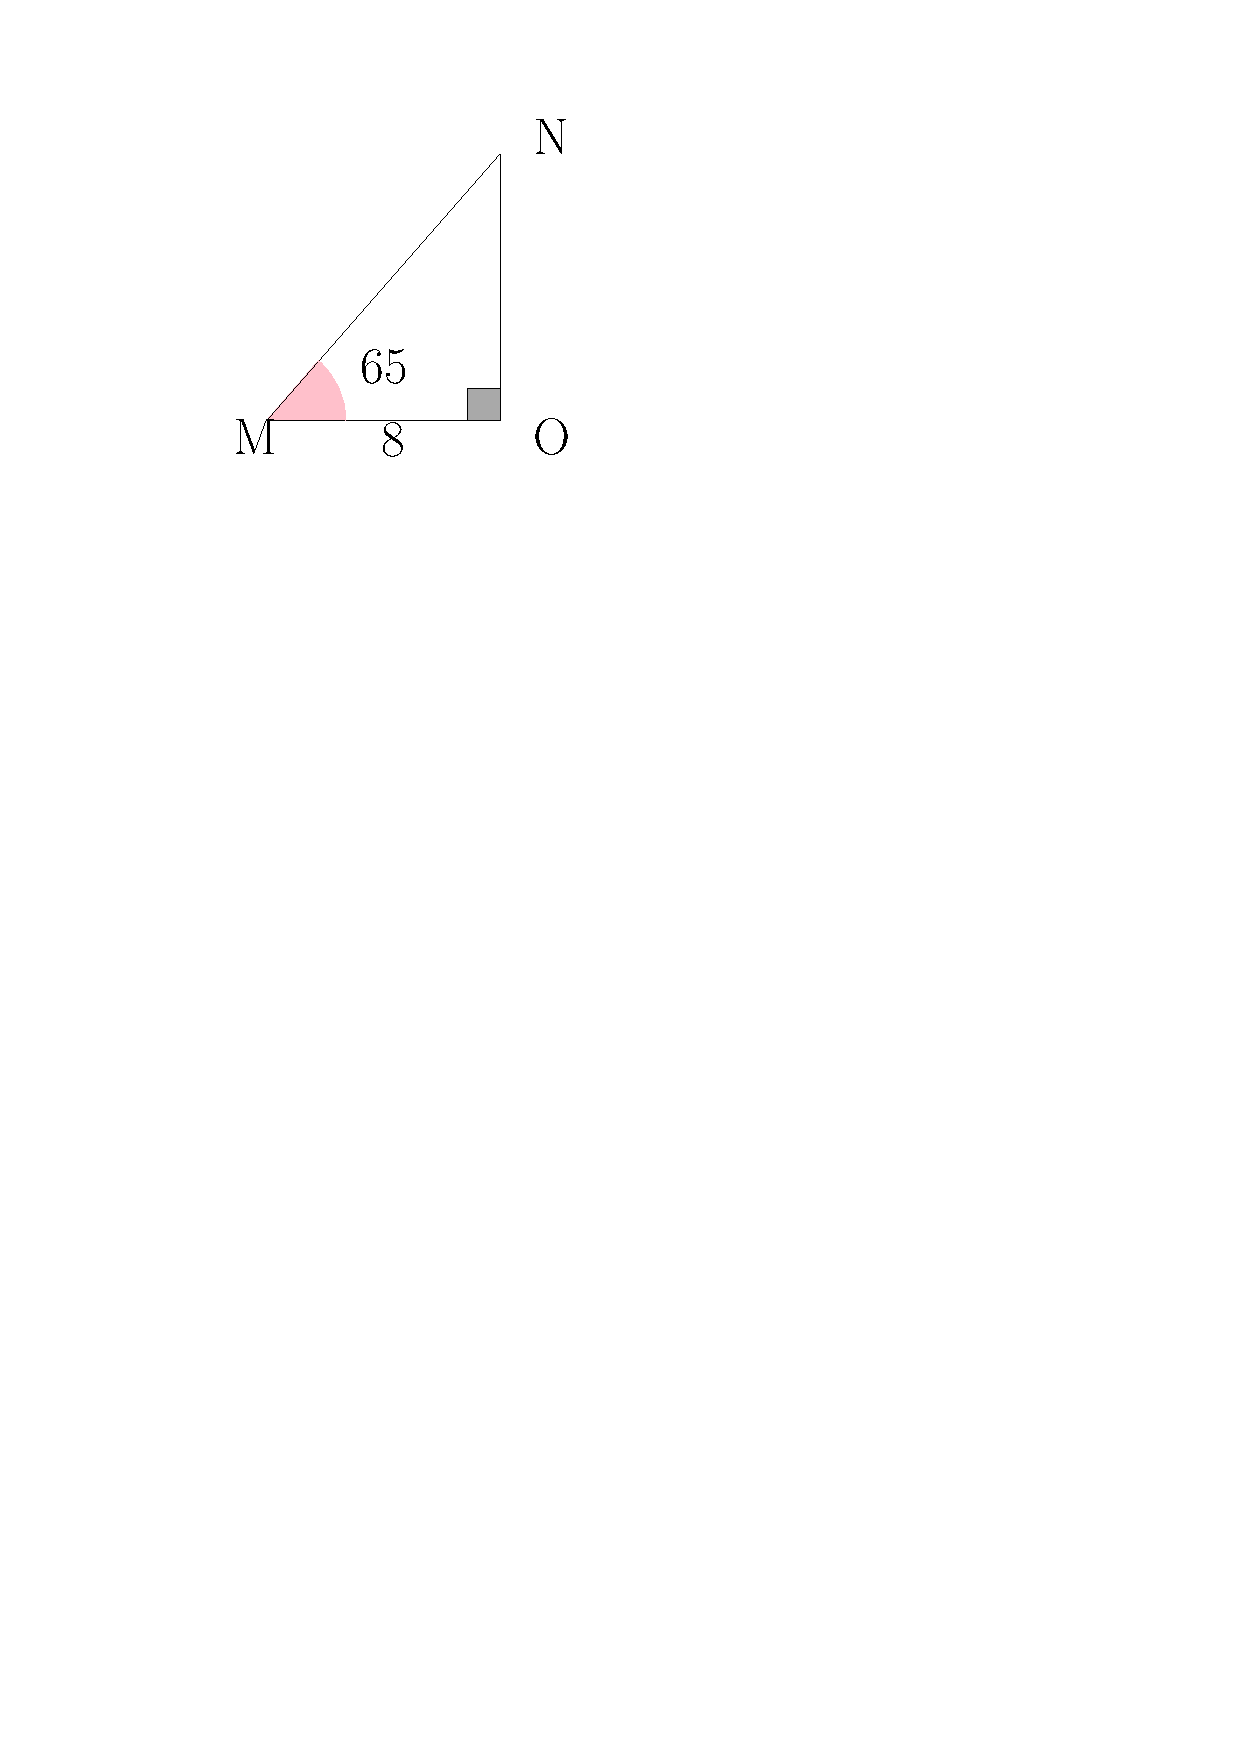
\includegraphics[width=\linewidth]{sources/2/rec-a2.pdf}
	    \end{figure}
      
      MNO est un triangle rectangle en O.\\
      
      $\cos(\overbrace{OMN}) = \dfrac{MO}{MN}$\\  
      $\cos(65) = \dfrac{8}{MN}$\\
      $MN \times \cos(65) = 8$\\
      $MN = \dfrac{8}{\cos{65}}$\\
      $MN \approx 18.9 $
      
    \end{multicols}
  \end{exampleblock}
  
\end{frame}

\begin{frame}
  \frametitle{{\rmfamily{\textsc{II - U}}}sages}

  B) Trouver la mesure d'un angle dans un triangle rectangle

  \begin{exampleblock}{Recherche de l'angle $\overbrace{ACB}$} 
    
    \begin{multicols}{2}

      \begin{figure}[H]
	      \centering
	      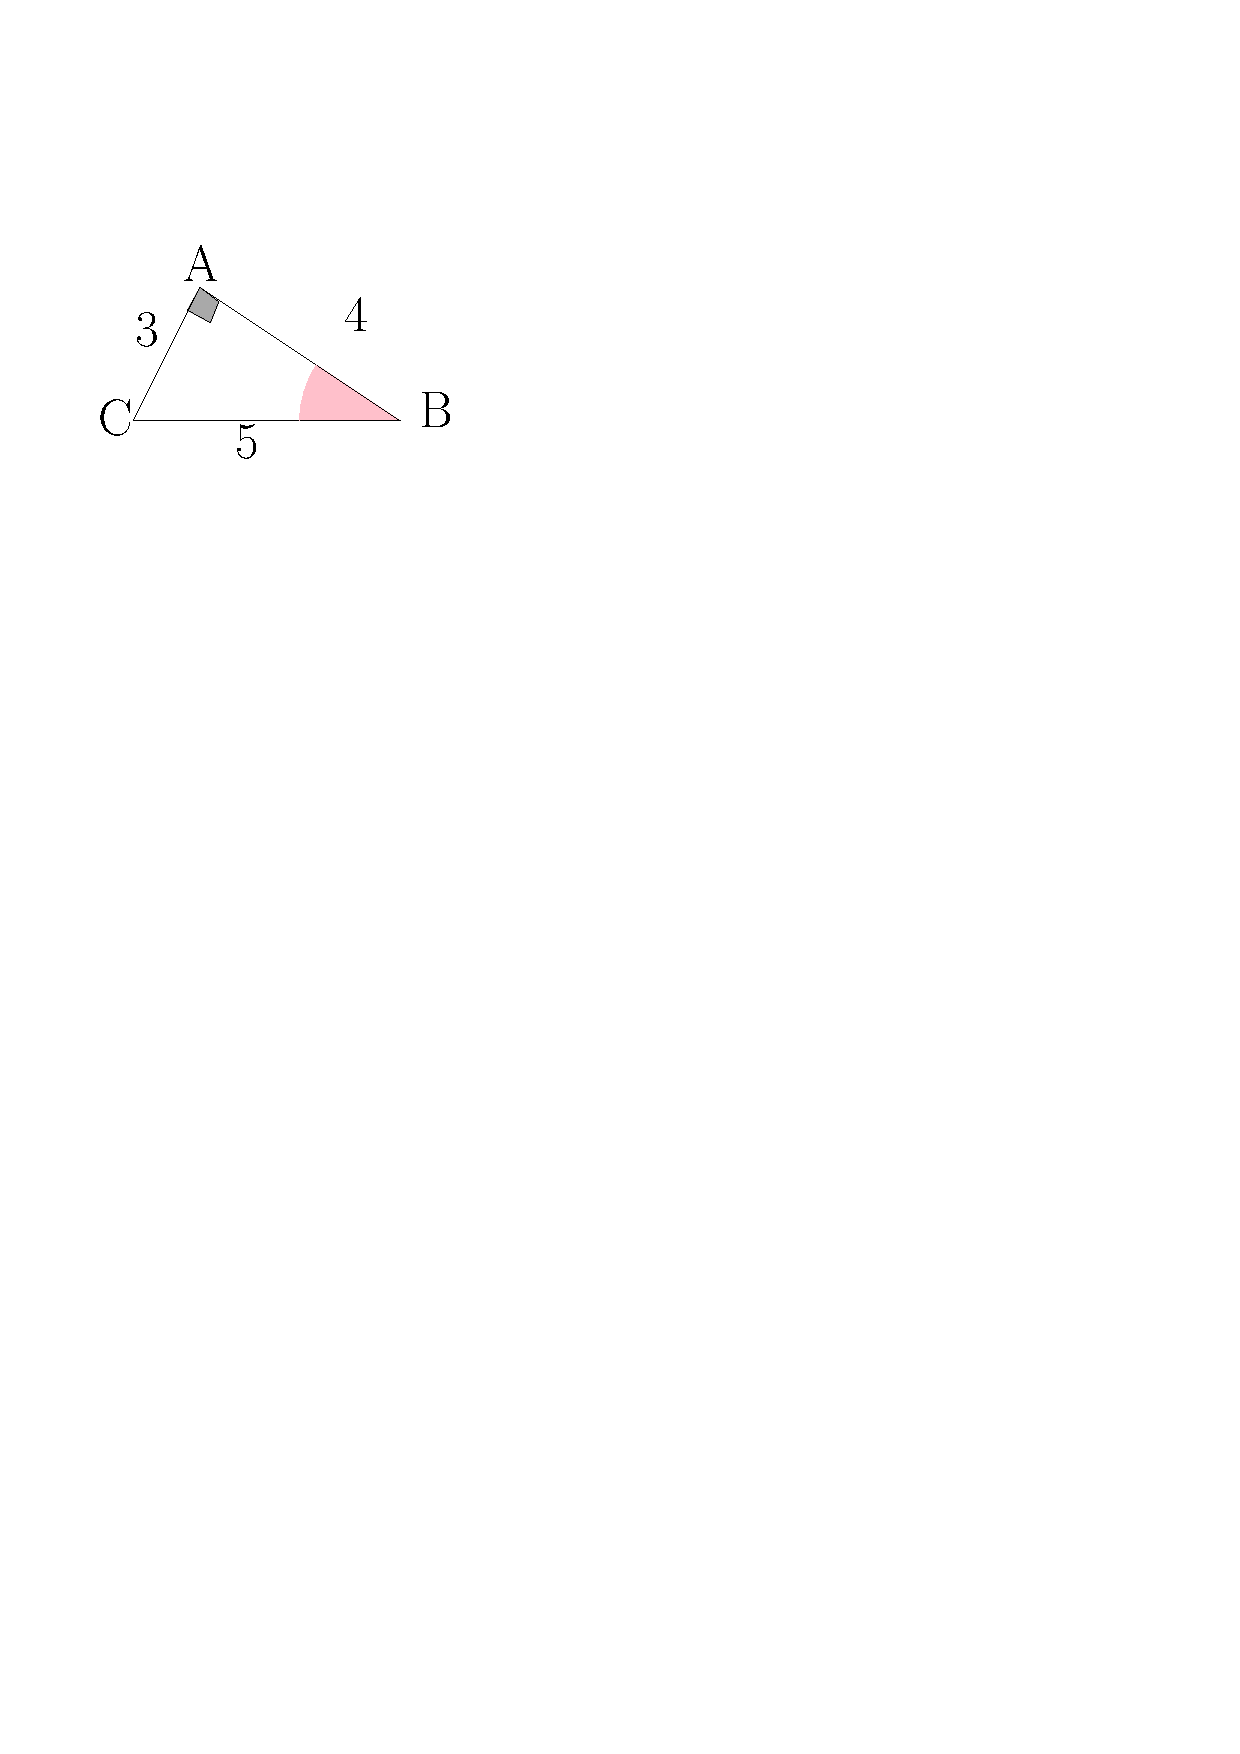
\includegraphics[width=\linewidth]{sources/2/rec-a3.pdf}
	    \end{figure}

      $\cos(\overbrace{ACB}) = \dfrac{CA}{CB}$\\
      $\cos(\overbrace{ACB}) = \dfrac{3}{5}$\\
      $\overbrace{ACB} = \cos^{-1} \left( \dfrac{3}{5} \right)$\\
      $\overbrace{ACB} = 53.1$
      
    \end{multicols}
  \end{exampleblock}  
  
\end{frame}

\begin{frame}
  \frametitle{{\rmfamily{\textsc{II - U}}}sages}

  \begin{block}{Remarques} 
    \begin{itemize}
    \item Il faut que la calculatrice soit bien en \textbf{degré}.
    \item Il faut faire attention aux \textbf{parenthèses}.
    \end{itemize}
      
  \end{block}  
  
\end{frame}

\end{document}
